%************************************************
\chapter{Un modèle morphologique de scènes sonores environnementales}\label{ch:psycho_model} % $\mathbb{ZNR}$
%************************************************

\section{Motivations}

\subsection{Analyse sensorielle}

étude de la contribution des sources sonores \\

G1: \citep{bruce2009development,bruce2014effects}; \\
G2: \citep{davies2014soundscape} montre que quand on demande à des participants de simuler un paysage sonore, les simulations font références à ce que les participants s'imaginent être un environnement typique, sans tenir compte de leur propre préférence pour des sons particuliers.

\subsection{Analyse automatique}

\section{Proposition d'un modèle de scènes sonores}

\subsection{Discrétiser l'environnement sonore}

\subsubsection{L'unité de bases: la source sonore}

Les études portant su l'ASA et plus spécifiquement sur les processus de ségrégation montrent que l'humain fait sens de son environnement en isolant les informations relatives aux différentes sources qui composent la scène. Elles montrent notamment que ce groupement intervient très tôt dans la chaîne de traitement, et se base sur des règles génériques innées. \\

\gl{Neurosciene}

De même, la communauté des paysages sonores, adoptant l’approche catégorielle, a également montré que les processus de catégorisation s'appuie également sur la composition sémantique des scènes,\ie~les sources sonores identifiées.

Il semble alors intuitif pour notre modèle de considérer comme élément de base la source sonore. Hors comme nous l'avons vu précédemment (\cf~section~ref{XX}), la notion de source sonore est variable, un même objet pouvant être reconnu suivant plusieurs degré d'abstraction.

\subsubsection{Typologie: source et action}

Avant de pouvoir enregistrer ces sources, il est nécessaire de les identifier. Une approche naïve serait alors d'établir la liste exhaustive de toutes les classes de sources sonores composant l'environnement sonore. Cette approche soulève alors 2 problèmes:

\begin{itemize}
\item Une source sonore peut se décrire avec plusieurs niveaux d'abstraction. Comme nous l'avons vu, identifier et nommé un objet est très lié à notre représentation mentale du monde. Selon la théorie de la catégorisation, l'organisation catégorielle de nos représentations se déploient, entre autre, selon un axe verticale, relatif au niveau d'abstraction considéré pour catégoriser un objet perçu. Ainsi, si 2 individus entendent un même son de voiture, il est possible que le premier le nomme ``\,voiture\,'' et le deuxième ``\,moteur\,''. Le dénombrement de l'ensemble des sources pouvant être utilisée par le modèle doit prendre en compte ce fait. Ces sources doivent être regroupée en classes hiérarchisée, afin de bâtir une structure taxonomique.
\item Il n'existe pas de taxonomie standardisé des sources sonores: C'est une tradition des sciences moderne de classer et nommer les différents objets d’intérêt avant de les étudier. Pour ce qui est de la faune ou de la flore, une observation longue et minutieuse ds objets a permis d'élaborer un système de classification standard, permettant d'organiser et trier les différents objets en fonction de leurs propriétés partagées. Les classes d’objets équivalents étant nommé à l'aide d'une terminologie précise. Ce système a permis à la biologie de devenir une science moderne à part entière, et entre autre de mettre à jour le concept de l'évolution des espèces \citep{lecointre2006tree}. Cependant, que ce soit pour les catégories d'odeurs ou les catégories de sons, il n’existe pas de système de classification équivalent \citep{dubois2000categories,niessen2010categories}. Nous isolons trois points qui permettent d'expliquer ce fait
\begin{itemize}
\item \emph{Champ lexical limité}: L'identification et la description d'un son est un processus subjectif très lié au langage. Deux sujets appartenant à deux groupes sociaux différents n'utiliseront pas les mêmes termes pour décrire un même son. Afin d'établir un système de classification standard, il faut prendre une décision quant à la définition précise des termes utilisés pour décrire les phénomènes acoustiques. Cette opération est d'autant plus facile si il existe déjà un consensus autour du sens global des termes. Or, contrairement à la vision, où un vocabulaire de base, largement partagé, est disponible pour décrire les objets (couleur, forme), il s'avère que le champ lexical utilisé pour décrire précisément le monde sonore est très limité (durée, fréquence)  \citep{dubois2000categories}. La plupart des termes couramment utilisés sont  empruntés à d'autres modalités perceptives. On peut par exemple parler de brillance ou de rugosité des sons. La diversité des termes descriptifs, ainsi que l'absence de consensus sur ce qu'ils désignent, rend difficile la production d'une classification standardisée des sons.
\item \emph{Influence du contexte}: Comme vu à la section~\ref{sec:ch3_identification et Contexte}, l'identification et la description d'une source sont dépendantes du contexte, \ie~de la nature des sources cooccurrentes dans la scènes \citep{ballas1987interpreting,niessen2008disambiguating,gygi2011incongruency}.
\end{itemize}
\end{itemize}

Il apparaît clairement que les classes de sons peuplant notre environnement doivent être organisée autour d'une taxonomie: un système de classe hiérarchisé. Cependant il y a un choix à faire quant à la manière de regrouper les sons à l'intérieur de cette taxonomie.

Comme vu à la section~\ref{XX}, plusieurs études ont montré que la catégorisation de sources sonores s'opère suivant des attributs sémantiques. Parmi ceux-ci, deux reviennent souvent:

\begin{itemize}
\item La source (agent, objet, fonction),\ie~l'objet émettant son.
\item L'action,\ie~le mouvement physique étant la cause du son.
\end{itemize} 

Ces deux attributs fonctionnent de concert. Reprenant l'organisation catégorielle verticale à trois niveaux de Rosch (\cf~section~\ref{sec:ch3_categoEtAbstract}), Guyot et al. \citep{guyot1997} ont proposé un système de catégorisation ou les auditeurs identifient des groupement de sources abstraits au niveau superordonné (``\,Bruit généré par une excitation mécanique\,''), des actions au niveau de base (``\,gratter\,'',``\,frotter\,'') et des sources au niveau subordonné (``\,vaisselles\,'',``\,stylo\,''). Reprenant ce système, \citep{houix_lexical_2012} montre que les sons semblent être catégorisés en premier à partir du type de source, et seulement ensuite sur la base de l'action.


Le couple source-action semble être une bonne base sur laquelle bâtir une taxonomie. Les classes haut-niveaux étant des classes abstraites de sources sonores (``\,véhicule\,''), les classes intermédiaires des classes de sources sonores (``\,voiture\,''), et les classes basses des actions sonores (``\,passage\,''). Pour les classes de bas-niveau, la variabilité intra-classe est alors minimale.

Considérer un couple source-action n'est cependant pas suffisant. Le choix des labels utilisés doit faire l'objet d'une sélection particulière. C'est label doivent être génériques, compréhensible, et décrire de manière non ambiguë les objets de la classe. Afin de les choisir, on peut se référer aux travaux de Gaver \citep{gaver1993world} qui propose une taxonomie phénoménologique des sons, de Niessen~\al \citep{niessen2010categories} qui établissent la liste des catégories sonores les plus utilisées à partir d'une étude bibliographique de 166 papiers, et plus récemment les travaux de Salamon~\al \citep{Salamon14}, qui propose une taxonomie de sons urbains, utilisant également le couple objet-action, et établie sur la base entre autre des travaux de brown~\al \citep{brown2011towards}.

Dans cette partie, nous montrons que  l'utilisation de la nomenclature basée sur le couple action-source nous permet de dénombrer et trier l'ensemble des sons présents dans l'environnement sonore.

Dans un cas pratique, il s'agirait alors, sur la base de la taxonomie établie, d'enregistrer pour chacune des classes  un nombre de sons suffisant. Considérant des environnements dense comme la ville ou la forêt, c'est approche pose des problèmes pratiques de faisabilité évidents. On peut cependant se demander si il est nécessaire d'enregistrer de manière séparé toutes les sources,\eg~doit on additionner plusieurs sons de voix pour simuler un son de foule ? Si oui, la diversité d'enregistrement nécessaire pourrait être considérable, le cerveau humain étant très sensible à la répétition de sons identiques \citep{agus2010rapid}.

Afin de contourner le problème, on peut là encore s’appuyer sur des considérations perceptives afin d'établir, dans un contexte expérimentale donné, quels sons requiert d'être enregistré séparément, et quels groupes de sons peuvent être enregistrer ensemble

\subsubsection{événements, textures et scènes amorphes}

Tout les sons n'ont pas le même intérêt. Typiquement, une voix humaine pourra facilement être isolée du reste des sons concurrents \citep{carlyon2004brain}. De même, un fond sonore de trafiques urbains sera moins informatif que d'autre sons ponctuels et proches~\citep{southworth1969sonic}.

Comme vu à la section~\ref{sec:ch3_catsoundscape}, Maffiolo montrent l'existence de deux processus cognitives distincts dont l'activation dépend de la nature des environnements: pour les scènes amorphes,\ie~sans événement apparent, les scènes sont analysées de manière holistique, alors que des scènes événementielles, \ie~comportant des événements identifiables, sont analysées de manière descriptive, sur la base d'une information sémantique extraite a partir des événements reconnus.

Ces résultats nous amène à penser que les processus de ségrégation dépendent également de la nature structurelle de l'environnement. Lorsqu'un des événements émergent de la mixture, le cerveau traite l'information des différentes sources de manière séparée. Plusieurs flux auditifs sont ainsi générés, \ie~un pour chaque séquence d'événements émis par la même source. A l'inverse, quand le cerveau ne parvient pas à isoler d'événement, la scène est traité globalement,\ie~tout ces éléments étant aggloméré dans un même flux. 

De même, les différents travaux sur les textures sonores (\cf~section~\ref{sec:ch3_eventTexture}), montrent que le cerveau a tendance à tendance à résumer l'information extraite lorsqu'il détecte qu'une séquence n'est  composée que d'un mélange de sons similaires et n'apporte pas d'information au cours du temps. 

Outre les événements sonores, deux autres types de sons semblent pouvoir être isolés:

\begin{itemize}
\item \emph{Scène amorphes}: un son contenant une faible information sémantique et analysé de manière holistique.
\item {Texture sonores}: un son dont les caractéristiques physiques restent stables au cours de temps et traité par le cerveau à partir de statistiques extraites d'une représentation temps-fréquence.
\end{itemize}

Nous pensons qu'il existe des connexions entre les notions de textures/événements, et celles des scènes amorphes/événementielles. Les séquences événementielles peuvent être vues comme des séquences composées soit uniquement d'événements, soit d'événements et de textures, la présence d'événements, porteurs d'une information plus riche, primant sur la nature des processus mis en œuvre. 

De même, les textures et les scènes amorphes sont traitées de manière holistique, à partir de propriétés acoustiques globales pour les scènes amorphes \citep{dubois2006cognitive,maffiolo_caracterisation_1999}, et sur la base d'une information résumée statistiquement pour les textures\citep{mcdermott2013summary}. Toutes deux portent par ailleurs une information limitée \citep{saint1995classification,nelken2013ear}. Cependant, les séquences amorphes sont spontanément décrites par des sujets comme des ``\,fonds sonores\,'' \citep{maffiolo_caracterisation_1999,guastavino2006ideal}, impliquant que ces dernières n'existent que suite à un processus de construction de flux auditifs, alors que les textures sont des objets seulement définis sur la base de leur nature physique. Un exemple de texture souvent cité est le sons du ``\,galop\,'', qui selon le contexte peut très bien se retrouver au premier plan de la scène. 

Considérant cela, nous pensons qu'il est possible de considérer une scènes amorphe comme étant une texture, ses caractéristiques physique demeurant stables au cours du temps, et beaucoup de scènes amorphes (``\,brouhaha de rue\,'', ``\,brouhaha de trafic\,'') étant par ailleurs citées comme étant des textures. Cependant l'inverse, considérer une texture comme une scène amorphe, n'est pas forcément vrai.

Afin de limiter le nombre d'enregistrements nécessaires, il est donc possible d'enregistrer directement des mixtures de sons, à condition que ces dernières puissent être considérée comme des textures, la définition de cette dernière notion englobant les scènes amorphes.

\subsubsection{Discussion}

\subsection{Description du modèle morphologique}


\subsubsection{Séquence de sources sonores}

Dans le modèle proposé, la scène sonore est vu comme une somme de source sonores, ou autrement dit, ``\,un squelette d'événements sur un lit de textures\,'' \citep{nelken2013ear}. 

D'un point de vu pratique, ces éléments sonores sont enregistrés. L'enregistrement d'un son isolé, qu'il s'agisse d'un événement, ou d'une texture est appelé un \emph{sample}. 

\begin{mydef}
Un sample est un enregistrement d'un son isolé, qu'il s'agisse d'un événement, ou d'une texture.
\end{mydef}


Ces samples sont regroupés en classes de sons hiérarchisées, formant une taxonomie. Un exemple d'une partie d'une taxonomie comme utilisé par le modèle est donné figure ~\ref{fig:orgDb}. Les niveaux hiérarchique de la taxonomie sont appelé niveau d'abstraction.  Les classes ayant un niveau d'abstraction élevé illustre un regroupement conceptuels de samples ayant potentiellement des caractéristiques variés (\ie~{Humain}). Plus le niveau de la classe est bas, plus le groupement induit est précis, regroupant des samples similaires (\ie~\emph{voix-adulte-cri}). 

\begin{mydef}
Une classe est une collection de samples, ou une collection de sous-classes, en fonction du niveau d'abstraction considéré.
\end{mydef}

Les classes de niveau d'abstraction élevé sont nommés uniquement à l'aide de terme abstraits désignant de manière global les samples qu'elles regroupent (\eg~\emph{transport}), alors que les classes de bas niveau utilise la nomenclature source-action (\eg~\emph{voiture passe}). Les classes du dernier niveau correspondent à des collections de samples, considéré de facto comme équivalents les uns aux autres.

Chaque classe de son est enfin lié à une piste. Cette dernière peut être vue comme une séquence temporelle où sont positionnés les différents samples. La piste peut être vue comme la contrepartie simulée du flux auditif.

\begin{mydef}
Une piste est une séquence temporelle composée de sample appartenant à une même classe de sons.
\end{mydef}

La construction de la taxonomie (nombre de classes, nombre de niveau d'abstraction), dépend bien évidemment de la tâche considérée. 

\begin{figure}[bth]
        \myfloatalign
        
\includegraphics[width=.8\linewidth]{gfx/3}
       \caption{Organisation hiérarchique de la banque de sons isolés utilisée pour la simulation}\label{fig:orgDb}
\end{figure}

\subsubsection{Paramètre}

En suivant la terminologie précédemment introduite, une scène sonore est vue comme une somme de piste. Chaque piste étant une séquence temporelle, dont la structure est dépend d'une série de paramètres. Ainsi, le modèle ne propose pas d’interagir avec un sample en particulier, mais toujours avec une séquence de samples.

Nous isolons trois attributs permettant de contrôler un piste:

\begin{itemize}
\item \emph{Le niveau}: la moyenne/variance des niveaux des samples
\item \emph{L'espacement}: la moyenne/variance des espacements inter-onsets entre les samples
\item \emph{La duré}: le débuts et la fin de la piste
\end{itemize}

Le modèle fait une distinction explicite entre la gestion des pistes d'événements et de textures. En effet, la notion de texture ne peut se comprendre que pour un son continue. Une piste de texture est donc composée de samples concaténé les uns aux autres sans espacement. Ce dernier, dans le cas des textures, est un paramètre imposé, fixé à 0. 

Pour qu'une piste de texture soit ``\,plausible\,'', \ie~qu'on ne détecte pas de discontinuité flagrante, la piste doit être une séquence composé de samples provenant de la même source, et obtenu avec un matériel et des réglages identiques.

\subsubsection{Formalisation du modèle}
 
 Tout au long due nos travaux, nous avons utilisé plusieurs modèles ainsi que différents paramètres afin de simuler des scènes sonores. Nous formalisons dans cette partie une version générale du modèle proposé. Les divers modifications appliquées, quand elles existent, seront indiquées dans les sections adéquates (\cf~section~\ref{xx}).
 
La formalisation présentée vaut uniquement pour les classes d'événements sonores. Nous décrivons par la suite les diverses contraintes qui s'appliquent pour une classe de textures.
 
En considérant $s$, une scène composée de $C$ classes de sons, le modèle de $s$ se définit  comme suit:
 
 \begin{equation}
 s(n)=\sum_{i=1}^{C}p_i(n)
 \end{equation}

avec $n$ un indice temporel discret, et $p_i$ la piste correspondant à la classe $c_i$. La classe $c_i$ est composé de $\vert c_i\vert$ samples $c_{i,m}$, $1<m<\vert c_i\vert$. 

Une piste $p_i$ est définie comme une séquence de $n_i$ samples d'événement $e^k_i(n)$ ($k=(1,2,\ldots,n_i)$), choisis aléatoirement parmi les $\vert c_i\vert$ samples de la classe $c_i$. Considérant $\mathcal{U}(x,y)$, une distribution uniforme d'entiers allant de $x$ à $y$ ($x<y$), on a alors:

 \begin{equation}
 e^k_i=c_{i,\mathcal{U}(1,\vert c_i \vert)}
 \end{equation}

 Pour chaque piste $p_i$, un facteur d'amplitude est tiré aléatoirement à partir d'une distribution normale de moyenne $\mu^a_i$ et de variance $\sigma^a_i$. De même, les espacements inter-onsets sont tirés d'un distribution normale de moyenne $\mu^t_i$ et de variance $\sigma^t_i$. Les indices temporelles de début et de fin de chaque piste sont notés $u_i$ et $v_i$ respectivement. Formellement, une piste $p_i$ se définit comme suit:
 
\begin{equation}
\label{eq1}
p_{i}(n)= \sum_{j=1}^{n_i} \mathcal{N}(\mu^a_{i},\sigma^a_{i})c_{i, \mathcal{U} (1, |c_i|)}(n-n^j_i)
\end{equation}
\begin{equation}
\label{eq2}
n_i^j=n_i^{j-1} + \mathcal{N}({\mu^t_{i},\sigma^t_{i}})
\end{equation}

où $n_i^0=u_i$ par convention. Le signal d'une piste est définit de telle sorte que $p_i(n)=0$ si $n>v_i$. Les paramètres du modèle sont, $\mu^a_i$,  $\sigma^a_i$,   $\mu^t_i$,  $\sigma^t_i$, $u_i$ et $v_i$, et doivent être réglé pour chaque piste $p_i$.


Pour les textures, deux distinctions sont à observer avec le modèle comme définit précédemment: 

\begin{enumerate}
\item L'amplitude du signal ($\mu^a_i$,  $\sigma^a_i$) n'est seulement tirée qu'une seule fois, et la valeur est appliquée à tous les samples.
\item Afin d'éviter tout impression de discontinuité, deux samples de texture sont concaténé en considérant un certain recouvrement. Ce recouvrement est choisi afin de pouvoir appliquer un fondu enchaîné (\emph{cross-fade}) à valeur d'énergie constante entre les samples, et ce afin de donner l'illusion de continuité.
\end{enumerate}


\gl{a revoir avec mathieu et mathias}

\section{Du modèle à la simulation dans le cadre de l'analyse sensorielle: l'outil \emph{Simscene}}

Dans cette section nous présentons une version du modèle précédemment introduit, afin qu'il puisse servir de base à  un outils de simulation, nommé \emph{SimScene}, utilisable dans le cadre de l'analyse sensorielle des scènes sonores.

Nous commençons par proposer un paradigme expérimentale  décrivant le cadre applicatif des épreuves perceptives basées sur la simulation. Nous relions par la suite ce paradigme au modèle de scène sonore, et présentons les fonctionnalité de l'outil \emph{SimScene}.

\subsection{Proposition d'un protocole expérimental basé sur la simulation}


\begin{figure}[bth]
        \myfloatalign
        
\includegraphics[width=.8\linewidth]{gfx/1}
       \caption{TODO}\label{fig:paradigmeSimu1}
\end{figure}

\begin{figure}[bth]
        \myfloatalign
        \includegraphics[width=.8\linewidth]{gfx/2}
       \caption{TODO}\label{fig:paradigmeSimu2}
\end{figure}

\begin{figure}[bth]
        \myfloatalign
        
\includegraphics[width=.8\linewidth]{gfx/4}
       \caption{Etape de processus de simulation pour l'analyse sensorielle}\label{fig:etapeSimu}
\end{figure}


\subsection{Organisation des sons isolées}
\label{db_ui}



\subsection{Sélection des sons isolés}

\subsection{Processus de simulation et paramètres de contrôle}

\section{Du modèle à la simulation dans le cadre de l'analyse automatique}

%*****************************************
%*****************************************
%*****************************************
%*****************************************
%*****************************************
